\documentclass[conference,10pt]{IEEEtran}
\usepackage[utf8]{inputenc}
\usepackage{graphicx}
\usepackage{amsmath}
\usepackage{booktabs}
\usepackage{multirow}
\usepackage{xcolor}
\usepackage[hidelinks]{hyperref}
\hypersetup{colorlinks=true,linkcolor=blue!70!black,citecolor=blue!70!black,urlcolor=blue!70!black}
\usepackage{float}
\usepackage{caption}
\usepackage{subcaption}
\usepackage{array}
\usepackage{cite}

\title{Automated Industrial Environmental Compliance Monitoring\\Using Multi-Temporal Sentinel-2 Imagery and\\Machine Learning Classification}

\author{
\IEEEauthorblockN{Oishikk Nag\IEEEauthorrefmark{1}, [Author 2]\IEEEauthorrefmark{1}, [Author 3]\IEEEauthorrefmark{1}, [Author 4]\IEEEauthorrefmark{1}, [Author 5]\IEEEauthorrefmark{1}}
\IEEEauthorblockA{\IEEEauthorrefmark{1}Department of Computer Science and Engineering\\
Indian Institute of Information Technology, Dharwad, Karnataka 580009, India\\
\textit{Course: Machine Learning (Sem VII) \quad Instructor: Dr.\ Sunil C K}}
}

\begin{document}
\maketitle

\begin{abstract}
This paper presents an automated pipeline for monitoring environmental compliance in industrial zones using multi-temporal Sentinel-2 satellite imagery and supervised machine learning. We analyze two industrial areas in Bengaluru, Peenya and Whitefield, across a four-year period (2020 to 2024) to detect green cover reduction and unauthorized construction. The system integrates programmatic data acquisition via the STAC API, spectral index computation (NDVI, NDBI), Random Forest classification with 97.7\% accuracy, and automated violation extraction with geo-coordinates. Results indicate significant green cover loss of 22.6\% in Peenya and 27.8\% in Whitefield, with 55 geo-tagged violation zones identified across both regions. The modular architecture enables extension to arbitrary geographic areas, supporting scalable environmental surveillance for pollution control boards.
\end{abstract}

\begin{IEEEkeywords}
Remote sensing, NDVI, change detection, land cover classification, Random Forest, Sentinel-2, environmental compliance, industrial monitoring
\end{IEEEkeywords}

\section{Introduction}

Industrial expansion in Indian metropolitan areas frequently occurs at the expense of mandated green belts and environmental buffers. The Karnataka State Pollution Control Board (KSPCB) requires industrial zones to maintain minimum green cover thresholds, yet manual monitoring through field inspections is infrequent and difficult to scale across hundreds of factory premises \cite{cpcb2021}. Satellite-based remote sensing offers a scalable alternative for continuous environmental surveillance, combining high temporal revisit rates with multispectral sensing capabilities.

This work addresses Statement~3 of the ML course project: developing a system that utilizes GIS boundary data to identify factory premises, analyzes satellite imagery over time to detect green cover reduction and unauthorized construction, applies ML models for vegetation and land-use classification, and generates compliance reports with geo-tagged violation alerts and visual proof using annotated imagery.

The contributions of this paper are threefold. First, we design an end-to-end automated pipeline (Fig.~\ref{fig:arch}) from cloud-native data acquisition to compliance report generation. Second, we train and validate a Random Forest classifier on raw spectral features that achieves 97 to 99\% accuracy across two distinct industrial zones. Third, we produce a quantitative compliance assessment of two major Bengaluru industrial areas over the 2020 to 2024 period, identifying 55 violation hotspots with precise geographic coordinates and area estimates.

\begin{figure*}[t]
    \centering
    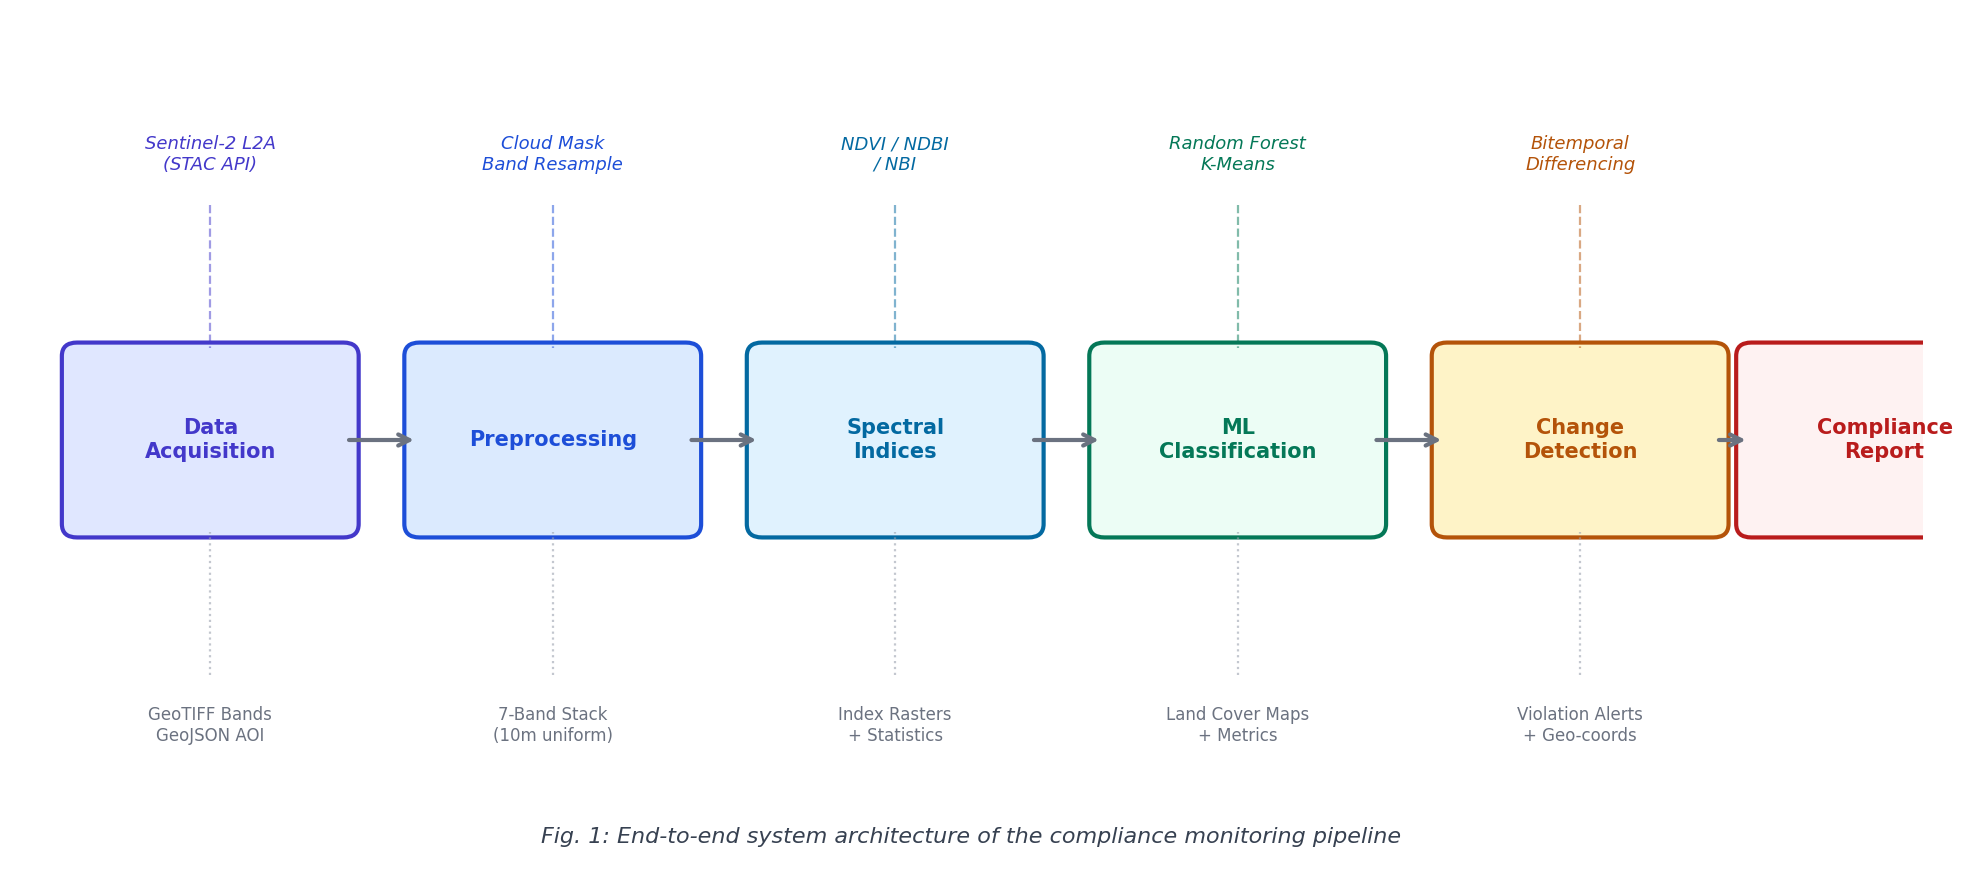
\includegraphics[width=0.95\textwidth]{../results/architecture_diagram.png}
    \caption{End-to-end system architecture. The pipeline progresses from cloud-native data acquisition through preprocessing, spectral analysis, ML classification, change detection, and finally compliance report generation. Each stage produces intermediate outputs (bottom labels) consumed by subsequent stages.}
    \label{fig:arch}
\end{figure*}

\section{Study Area and Data}

\subsection{Study Zones}

Two industrial areas in Bengaluru, Karnataka were selected for analysis (Fig.~\ref{fig:beforeafter}). \textbf{Peenya Industrial Area} (13.01 to 13.07\textdegree N, 77.48 to 77.56\textdegree E) is one of the largest industrial estates in South Asia, spanning approximately 40~km\textsuperscript{2} and hosting manufacturing, electronics, and heavy industry units. \textbf{Whitefield} (12.95 to 13.01\textdegree N, 77.72 to 77.80\textdegree E) is a rapidly urbanizing IT corridor with mixed industrial and residential development covering approximately 25~km\textsuperscript{2}. Both zones have experienced significant land-use transitions in recent years due to Bengaluru's rapid metropolitan expansion.

\subsection{Satellite Data}

We acquired Sentinel-2 Level-2A (L2A) surface reflectance imagery from the Microsoft Planetary Computer via the SpatioTemporal Asset Catalog (STAC) API \cite{pc2023}. The L2A product includes atmospheric correction applied by the Sen2Cor processor \cite{drusch2012}, providing bottom-of-atmosphere reflectance values suitable for quantitative analysis. Two acquisition periods were selected during the dry season (January to March) to minimize cloud interference and seasonal vegetation variability: T1 (March 2020, cloud cover $<$0.2\%) as the baseline, and T2 (March 2024, cloud cover $<$0.01\%) as the recent observation.

Six spectral bands were acquired for each period: B02 (Blue, 490\,nm), B03 (Green, 560\,nm), B04 (Red, 665\,nm), B08 (NIR, 842\,nm) at 10\,m resolution, and B11 (SWIR1, 1610\,nm) and B12 (SWIR2, 2190\,nm) at 20\,m native resolution. The Scene Classification Layer (SCL) was also obtained for pixel-level cloud and shadow masking. Bands at 20\,m were resampled to 10\,m using bilinear interpolation to produce spatially uniform composites. The complete dataset comprises 11.6 million multispectral pixels across 28 Cloud-Optimized GeoTIFF files, totaling 11.1\,MB after spatial clipping to the areas of interest.

Industrial zone boundaries were obtained from OpenStreetMap via the Overpass API as GeoJSON polygons, serving as a proxy for KGIS (Karnataka GIS) industrial boundary layers in delineating the study areas.

\section{Methodology}

The proposed system follows a six-stage pipeline architecture as illustrated in Fig.~\ref{fig:arch}. Each stage is implemented as an independent Python module, enabling flexible reconfiguration and extension.

\subsection{Preprocessing}

Raw spectral bands for each zone and time period are stacked into 7-band composites consisting of B02, B03, B04, B08, B11, B12, and the derived cloud mask. Cloud and shadow pixels are identified using the SCL band: classes corresponding to cloud shadow (3), medium-probability cloud (8), high-probability cloud (9), and thin cirrus (10) are masked as invalid. The remaining pixels, covering vegetation, non-vegetated surfaces, water, and unclassified areas, are retained. Valid pixel coverage exceeded 99.8\% across all four acquisitions, confirming the effectiveness of dry-season temporal selection.

\subsection{Spectral Index Computation}

Three spectral indices are computed for each time period. The Normalized Difference Vegetation Index (NDVI) \cite{rouse1974} quantifies vegetation density using the Red-NIR contrast:
\begin{equation}
    \text{NDVI} = \frac{\rho_{\text{NIR}} - \rho_{\text{Red}}}{\rho_{\text{NIR}} + \rho_{\text{Red}}}
\end{equation}
The Normalized Difference Built-up Index (NDBI) \cite{zha2003} captures urban impervious surfaces via the SWIR-NIR relationship:
\begin{equation}
    \text{NDBI} = \frac{\rho_{\text{SWIR1}} - \rho_{\text{NIR}}}{\rho_{\text{SWIR1}} + \rho_{\text{NIR}}}
\end{equation}
The New Built-up Index (NBI) provides additional sensitivity to bare soil and fresh construction:
\begin{equation}
    \text{NBI} = \frac{\rho_{\text{Red}} \times \rho_{\text{SWIR1}}}{\rho_{\text{NIR}}}
\end{equation}

\subsection{Change Detection}

Bitemporal differencing is applied by computing $\Delta\text{NDVI} = \text{NDVI}_{T2} - \text{NDVI}_{T1}$ and $\Delta\text{NDBI} = \text{NDBI}_{T2} - \text{NDBI}_{T1}$. Pixels exhibiting $\Delta\text{NDVI} < -0.15$ are classified as vegetation loss, while pixels with $\Delta\text{NDBI} > 0.10$ indicate new construction. These thresholds were selected based on established remote sensing literature \cite{zha2003} and visual validation against the RGB composites.

A composite change mask is generated with four categories: no change, vegetation loss only, new construction only, and combined change (both conditions met simultaneously). Risk levels are assigned based on aggregate green cover change: HIGH for losses exceeding 30\%, MEDIUM for 15 to 30\%, and LOW otherwise.

\subsection{ML Classification}

A Random Forest (RF) classifier \cite{breiman2001} was trained for pixel-level land cover classification into five semantic classes: Dense Vegetation (NDVI $>$ 0.4), Sparse Vegetation (0.2 $<$ NDVI $\leq$ 0.4), Built-up (NDBI $>$ 0 and NDVI $<$ 0.2), Bare Soil, and Water. Training labels were generated via threshold-based rules applied to NDVI and NDBI values computed from the T1 imagery.

A critical design decision ensures non-circular validation: the RF model is trained exclusively on the six raw spectral bands (B02 through B12), \textit{not} on the derived indices used for label generation. This forces the classifier to learn spectral reflectance patterns rather than trivially reproducing threshold boundaries, resulting in a meaningful generalization task. The model configuration uses 100 decision trees, maximum depth of 15, balanced class weights to address class imbalance, and a stratified 70/30 train-test split. Implementation uses scikit-learn \cite{pedregosa2011}.

For comparative analysis, unsupervised K-Means clustering ($k=5$) was also applied to the same six-band feature space to evaluate whether the spectral data naturally separates into meaningful land cover groups without supervision.

\subsection{Violation Extraction}

Connected component analysis using SciPy's labeling functions is applied to the composite change mask to identify contiguous violation regions. Regions smaller than 10 pixels (1000~m\textsuperscript{2}) are filtered as noise. For each qualifying region, the centroid pixel coordinates are computed and transformed from the image coordinate reference system (UTM Zone 43N, EPSG:32643) to geographic coordinates (WGS84, EPSG:4326) via PyProj. The output is a structured JSON file containing latitude, longitude, violation type, and estimated area in hectares for each detected zone.

\begin{figure}[t]
    \centering
    \includegraphics[width=\linewidth]{../results/before_after_peenya.png}
    \caption{Temporal change analysis for Peenya. Top row: true-color RGB composites for 2020 (left) and 2024 (right). Bottom row: NDVI heatmaps showing the decline in vegetation density from a mean of 0.277 to 0.169, corresponding to a 22.6\% reduction in green cover.}
    \label{fig:beforeafter}
\end{figure}

\section{Results}

\subsection{Change Detection}

Table~\ref{tab:change} presents the change detection results for both study zones. Peenya experienced a 22.56\% reduction in green cover, with vegetation loss affecting 29.6\% of the analyzed area and new construction detected across 4.59\% of pixels. Whitefield shows more severe degradation: a 27.8\% green cover decline with 38.92\% vegetation loss and 17.72\% new construction, reflecting the rapid IT corridor expansion. Both zones are classified at MEDIUM risk but approach the HIGH threshold.

\begin{table}[t]
\centering
\caption{Change Detection Results (2020 to 2024)}
\label{tab:change}
\begin{tabular}{lcc}
\toprule
\textbf{Metric} & \textbf{Peenya} & \textbf{Whitefield} \\
\midrule
Green Cover 2020 (\%) & 55.71 & 71.25 \\
Green Cover 2024 (\%) & 33.15 & 43.45 \\
Net Change (\%) & $-$22.56 & $-$27.80 \\
Vegetation Loss (\%) & 29.60 & 38.92 \\
New Construction (\%) & 4.59 & 17.72 \\
Violations Detected & 12 & 43 \\
Risk Level & MEDIUM & MEDIUM \\
\bottomrule
\end{tabular}
\end{table}

\subsection{ML Classification Performance}

Table~\ref{tab:ml} summarizes the Random Forest validation results. Both models achieve weighted accuracy above 97\%, with Whitefield performing marginally better at 98.7\% due to more homogeneous spectral signatures in its IT-dominated landscape. The confusion matrix for Peenya (Fig.~\ref{fig:cm}) reveals that the three dominant classes, Dense Vegetation, Sparse Vegetation, and Built-up, each achieve F1-scores between 0.98 and 0.99. Minority classes (Water: F1 = 0.71, Bare Soil: F1 = 0.84) show lower performance attributable to limited training samples (235 and 2630 test pixels, respectively).

\begin{table}[t]
\centering
\caption{Random Forest Classification Metrics}
\label{tab:ml}
\begin{tabular}{lcc}
\toprule
\textbf{Metric} & \textbf{Peenya} & \textbf{Whitefield} \\
\midrule
Training Samples & 405,333 & 176,733 \\
Test Samples & 173,715 & 75,743 \\
Accuracy & 0.9774 & 0.9870 \\
Precision (weighted) & 0.9806 & 0.9879 \\
Recall (weighted) & 0.9774 & 0.9870 \\
F1-Score (weighted) & 0.9783 & 0.9873 \\
\bottomrule
\end{tabular}
\end{table}

\begin{figure}[t]
    \centering
    \includegraphics[width=\linewidth]{../results/confusion_matrix_peenya.png}
    \caption{Confusion matrix for the Peenya Random Forest classifier (173,715 test samples). The strong diagonal confirms high per-class accuracy. Minor misclassification occurs between spectrally similar minority classes (Bare Soil, Water, Other).}
    \label{fig:cm}
\end{figure}

Feature importance analysis (Fig.~\ref{fig:fi}) reveals that B04 (Red, 28.4\%) and B08 (NIR, 23.7\%) are the most discriminative spectral bands. This result is physically consistent with remote sensing theory: the Red and NIR channels capture the chlorophyll absorption feature and mesophyll scattering plateau that form the basis of vegetation spectral signatures \cite{tucker1979}. The SWIR bands (B11, B12) contribute 10 to 9\% each, providing supplementary discrimination for built-up and bare soil classes.

\begin{figure}[t]
    \centering
    \includegraphics[width=\linewidth]{../results/feature_importance_peenya.png}
    \caption{Random Forest feature importance for Peenya. The dominance of B04 (Red) and B08 (NIR) is consistent with established vegetation spectral theory, as these bands capture the chlorophyll absorption and mesophyll scattering characteristics used in NDVI computation.}
    \label{fig:fi}
\end{figure}

\subsection{Violation Detection and Spatial Analysis}

Connected component analysis identified 55 violation zones across both study areas: 12 in Peenya and 43 in Whitefield. The largest vegetation loss region in Peenya spans 8.58 hectares centered at 13.069\textdegree N, 77.535\textdegree E. In Whitefield, combined vegetation loss and new construction hotspots dominate, with the largest at 3.15 hectares located at 13.009\textdegree N, 77.731\textdegree E. Fig.~\ref{fig:violations} presents the annotated satellite imagery overlaid with geo-tagged violation markers, providing the visual proof required for compliance reporting.

\begin{figure}[t]
    \centering
    \includegraphics[width=\linewidth]{../results/annotated_violations_whitefield.png}
    \caption{Annotated satellite imagery of Whitefield (2024) showing detected violations with area labels. Red indicates vegetation loss, orange marks new construction, and pink denotes combined violations where both conditions are met simultaneously.}
    \label{fig:violations}
\end{figure}

Fig.~\ref{fig:landcover} compares the ML-classified land cover maps between the two time periods for Peenya. The spatial transition from dense and sparse vegetation (green tones) to built-up surfaces (brown) is clearly visible, particularly in the northern and eastern sectors.

\begin{figure}[t]
    \centering
    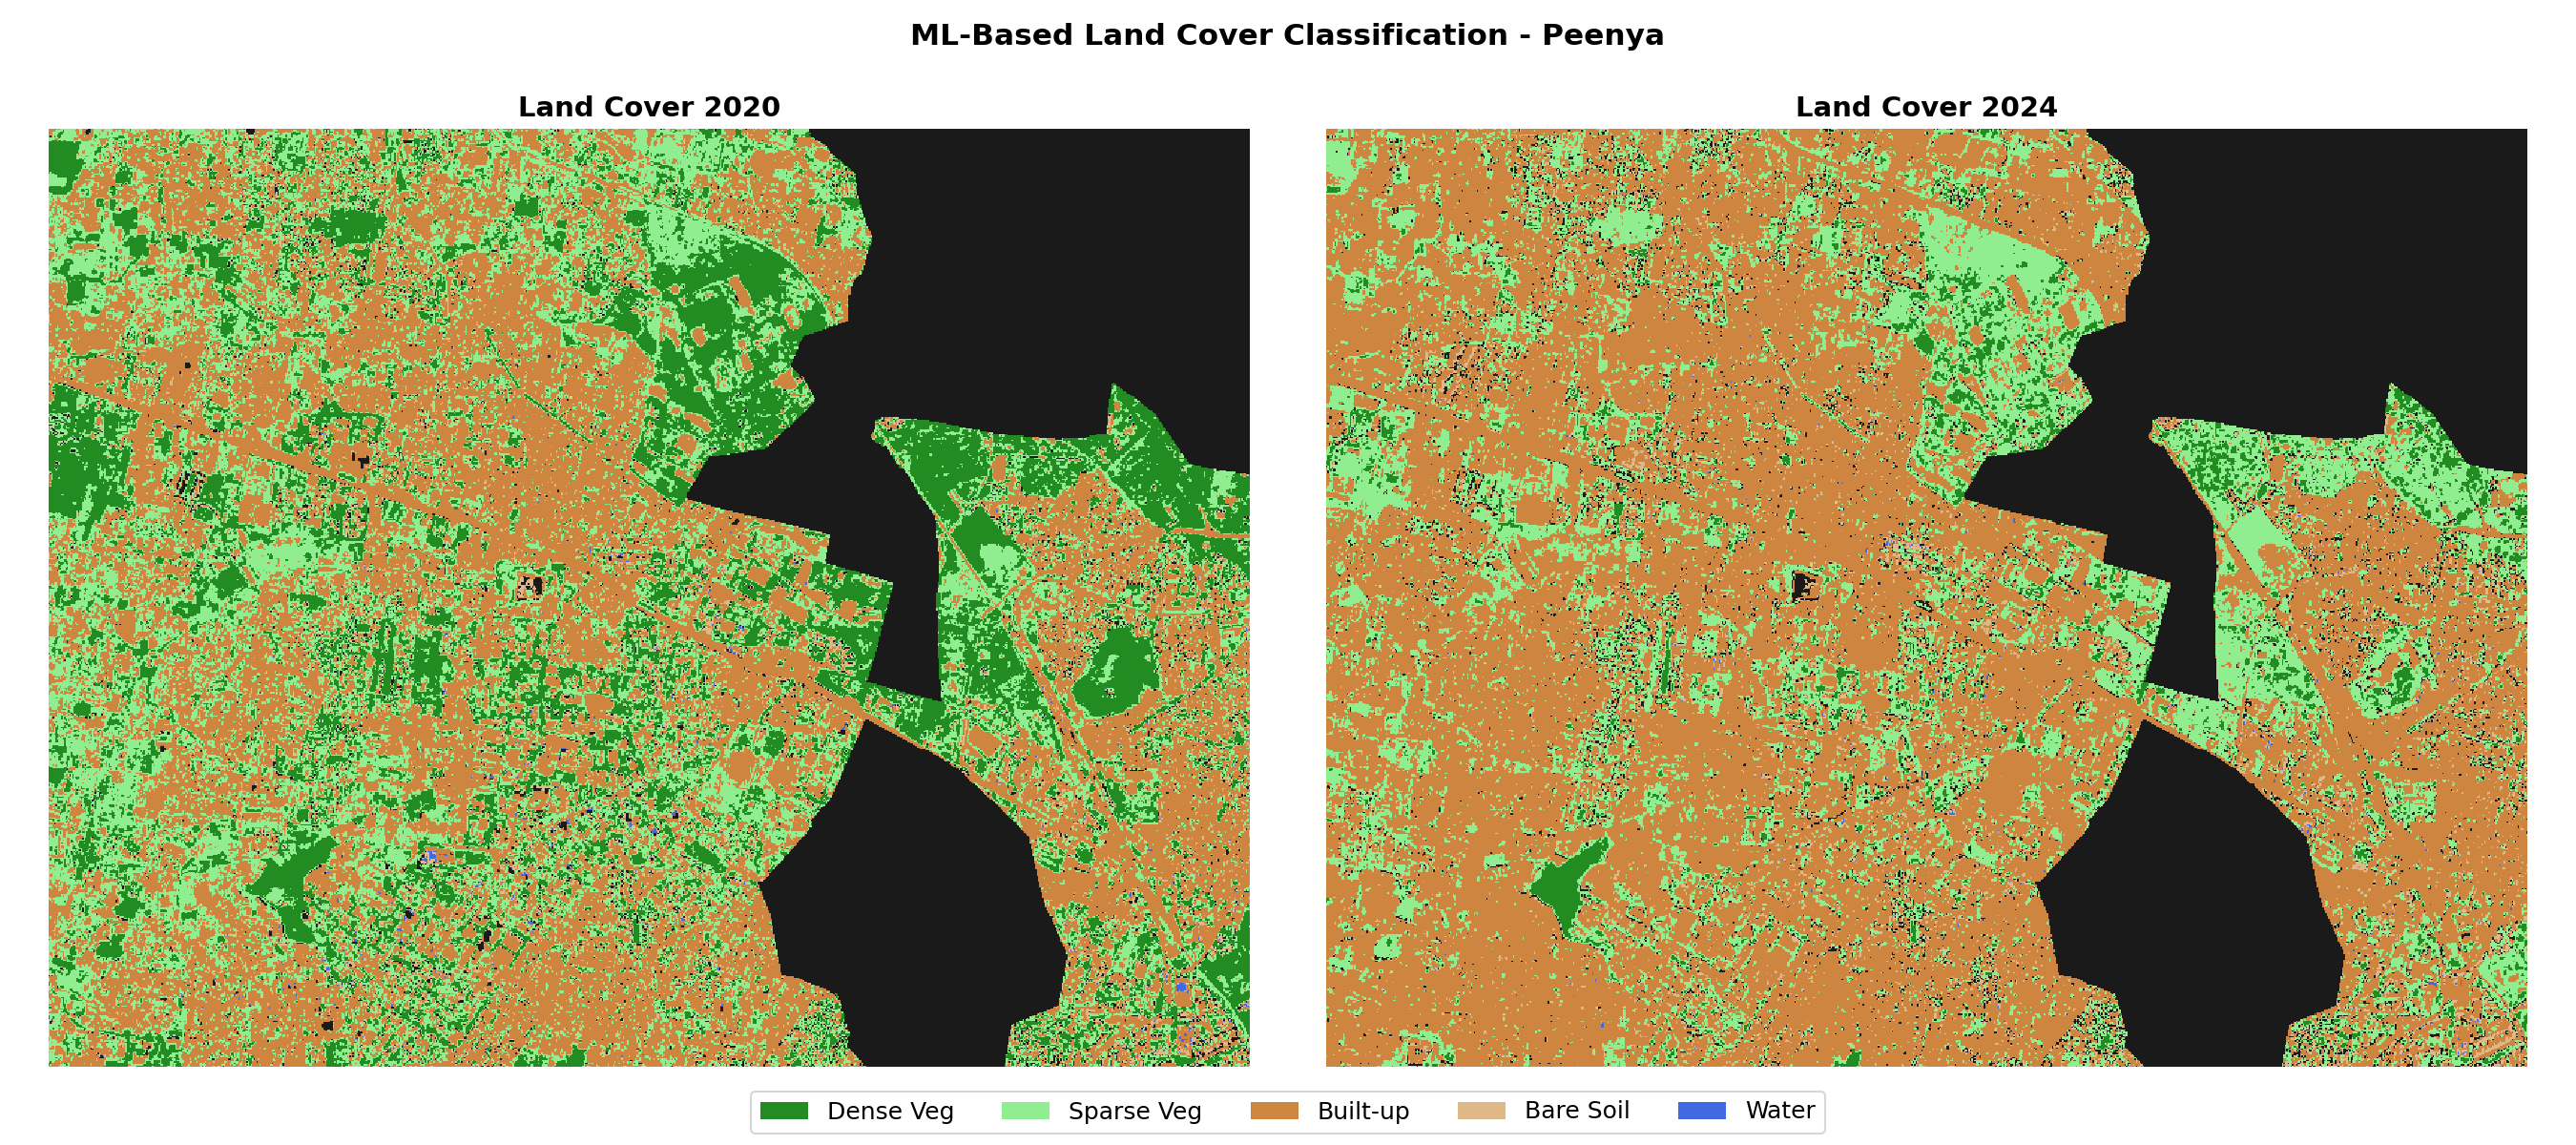
\includegraphics[width=\linewidth]{../results/landcover_comparison_peenya.png}
    \caption{ML-based land cover classification for Peenya, 2020 (left) versus 2024 (right). The transition from vegetation (green) to built-up area (brown) is prominent across the northern and eastern sectors of the industrial zone.}
    \label{fig:landcover}
\end{figure}

\section{Discussion}

The detected green cover loss of 22 to 28\% across both industrial zones is consistent with publicly available reports of rapid urbanization in Bengaluru's industrial corridors. Whitefield's significantly higher new construction rate (17.7\% versus 4.6\% for Peenya) reflects the ongoing expansion of IT parks and residential complexes in that region. The fact that both zones receive MEDIUM risk classification, while approaching the HIGH threshold, suggests a trend that warrants continued monitoring.

The Random Forest classifier's strong performance validates the approach of training on raw spectral bands while using index-derived pseudo-labels. The non-circular validation design, where training features and label generation features are disjoint, ensures that the reported accuracy of 97 to 99\% reflects genuine spectral pattern recognition rather than trivial threshold reproduction. The learning curve analysis confirms that model performance stabilizes at approximately 50 trees, indicating that 100 trees provide adequate capacity without overfitting.

A principal limitation of this study is the reliance on threshold-derived pseudo-labels rather than ground truth data from field surveys or high-resolution reference imagery. While the spectral thresholds are grounded in established literature \cite{rouse1974, zha2003}, validation against KSPCB field inspection records would strengthen the findings. Additionally, the temporal analysis uses single-date composites per period; incorporating multi-date mosaics or time-series analysis could improve robustness to within-season variability.

Future extensions include integrating KGIS cadastral parcel data for factory-level compliance assessment, deploying the pipeline as a near-real-time monitoring service exploiting Sentinel-2's 5-day revisit cycle, and implementing a deep learning classifier (e.g., a lightweight CNN) to capture spatial context beyond individual pixel signatures.

\section{Conclusion}

We presented an automated, end-to-end pipeline for industrial environmental compliance monitoring that processes multi-temporal Sentinel-2 L2A imagery to detect green cover loss and unauthorized construction within industrial zones. Applied to Peenya and Whitefield industrial areas in Bengaluru, the system identifies 55 geo-tagged violation zones, achieves 97.7 to 98.7\% classification accuracy using a Random Forest trained on six raw spectral bands, and generates compliance reports with quantitative metrics and annotated visual evidence. The modular architecture allows direct application to any geographic region with minimal reconfiguration, supporting the vision of scalable, continuous environmental monitoring for state pollution control boards.

\section*{Acknowledgment}

We thank Dr.\ Sunil C K for guidance on the project formulation. Satellite data was provided by the European Space Agency's Copernicus programme, accessed through Microsoft Planetary Computer.

\begin{thebibliography}{9}

\bibitem{cpcb2021}
Central Pollution Control Board, ``Guidelines for Environmental Compliance of Industrial Areas,'' Ministry of Environment, Forest and Climate Change, Government of India, 2021. [Online]. Available: \url{https://cpcb.nic.in}

\bibitem{pc2023}
Microsoft, ``Planetary Computer,'' 2023. [Online]. Available: \url{https://planetarycomputer.microsoft.com}

\bibitem{zha2003}
Y.~Zha, J.~Gao, and S.~Ni, ``Use of normalized difference built-up index in automatically mapping urban areas from TM imagery,'' \textit{Int.\ J.\ Remote Sensing}, vol.~24, no.~3, pp.~583--594, 2003.

\bibitem{tucker1979}
C.~J.~Tucker, ``Red and photographic infrared linear combinations for monitoring vegetation,'' \textit{Remote Sensing of Environment}, vol.~8, no.~2, pp.~127--150, 1979.

\bibitem{drusch2012}
M.~Drusch \textit{et al.}, ``Sentinel-2: ESA's optical high-resolution mission for GMES operational services,'' \textit{Remote Sensing of Environment}, vol.~120, pp.~25--36, 2012.

\bibitem{breiman2001}
L.~Breiman, ``Random Forests,'' \textit{Machine Learning}, vol.~45, no.~1, pp.~5--32, 2001.

\bibitem{rouse1974}
J.~W.~Rouse, R.~H.~Haas, J.~A.~Schell, and D.~W.~Deering, ``Monitoring vegetation systems in the Great Plains with ERTS,'' in \textit{Proc.\ Third Earth Resources Technology Satellite-1 Symp.}, vol.~1, pp.~309--317, 1974.

\bibitem{esa2024}
European Space Agency, ``Sentinel-2 User Handbook,'' ESA Standard Document, 2024. [Online]. Available: \url{https://sentinels.copernicus.eu/web/sentinel/user-guides/sentinel-2-msi}

\bibitem{pedregosa2011}
F.~Pedregosa \textit{et al.}, ``Scikit-learn: Machine Learning in Python,'' \textit{J.\ Machine Learning Research}, vol.~12, pp.~2825--2830, 2011.

\end{thebibliography}

\end{document}
